% =====================================================================
%  CricketMind -- Architecture Draft v4
%  Verified Claims over Real Evidence
%
%  Revision notes vs. v3:
%    * C7: a tone word is a hidden comparison and must be backed by a
%      checked comparison claim; new fabrication class F8.
%    * Every question gets an honest answer: five kinds of question, a
%      read-back, filters x measures in N8 M1, the Explainer (N11m) for
%      rules, and an honest decline for what no data can answer.
%    * False premises and trick attempts: N3 marks them, C7 checks them.
%    * A receipt for every number, taken from C2's own re-query.
%    * A sport-neutral Subject and a football case study.
%    * Perception through an exported model; N1 follows its model card.
%    * Claims check their own rules; displayed numbers round halves up.
%    * A journal-grade evaluation: locked exams, baselines, an ablation,
%      AI checkers, three models, an outside test set, a human study.
%
%  Status: the claim language (plan days 6-9) is built and tested; the
%  rest is design.  The codebase is still called cricketmind-v3.
%  Compile with: pdflatex CricketMind_Architecture_v4.tex   (run twice)
% =====================================================================
\documentclass[11pt,a4paper]{article}

\usepackage[margin=2cm]{geometry}
\usepackage[T1]{fontenc}
\usepackage[utf8]{inputenc}
\usepackage{lmodern}
\usepackage{booktabs}
\usepackage{array}
\usepackage{xcolor}
\usepackage{amsmath}
\usepackage{enumitem}
\usepackage{float}
\usepackage{capt-of}
\usepackage[section]{placeins}
\usepackage[font=small,labelfont=bf,hypcap=false]{caption}
\usepackage{tikz}
\usetikzlibrary{shapes.geometric,arrows.meta,positioning,calc,fit,backgrounds}
\usepackage[hidelinks]{hyperref}
\def\UrlBreaks{\do\/\do-\do\_}
\setlength{\emergencystretch}{1.5em}
\renewcommand{\topfraction}{0.85}
\renewcommand{\textfraction}{0.1}
\renewcommand{\floatpagefraction}{0.75}
% a table or figure with its caption, never split across pages
\newenvironment{keep}{\par\medskip\noindent\begin{minipage}{\textwidth}\centering}{\end{minipage}\par\medskip}

% ---------------------------------------------------------------- colours
\definecolor{encblue}{RGB}{31,58,110}      % vision / text encoding
\definecolor{fuseteal}{RGB}{17,110,110}    % multimodal fusion
\definecolor{retbrown}{RGB}{124,76,38}     % retrieval
\definecolor{svcorange}{RGB}{176,90,20}    % sanctioned engines
\definecolor{routeviolet}{RGB}{88,48,132}  % supervisor / router
\definecolor{agentgreen}{RGB}{27,94,58}    % stakeholder agents
\definecolor{gatered}{RGB}{170,30,40}      % confidence gate
\definecolor{gatepurple}{RGB}{112,44,132}  % faithfulness gate
\definecolor{dbtan}{RGB}{222,196,160}      % databases
\definecolor{outgrey}{RGB}{45,45,50}       % final output
\definecolor{gateslate}{RGB}{72,88,104}    % entry branch
\definecolor{newgold}{RGB}{214,160,20}     % new or changed in v4

% ---------------------------------------------------------------- styles
\tikzset{
  base/.style   = {draw, rounded corners=2pt, align=center, font=\small,
                   minimum width=2.9cm, minimum height=1.1cm, inner sep=3pt,
                   line width=0.7pt},
  enc/.style    = {base, fill=encblue,     text=white, draw=encblue!55!black},
  fuse/.style   = {base, fill=fuseteal,    text=white, draw=fuseteal!55!black},
  ret/.style    = {base, fill=retbrown,    text=white, draw=retbrown!55!black},
  svc/.style    = {base, fill=svcorange,   text=white, draw=svcorange!55!black},
  route/.style  = {base, fill=routeviolet, text=white, draw=routeviolet!55!black},
  agent/.style  = {base, fill=agentgreen,  text=white, draw=agentgreen!55!black,
                   minimum width=2.7cm, minimum height=1.2cm, font=\footnotesize},
  outnode/.style    = {base, fill=outgrey,     text=white, draw=black},
  gate/.style   = {draw, diamond, aspect=2.0, align=center,
                   font=\footnotesize\bfseries, inner sep=2pt, line width=0.7pt},
  confgate/.style  = {gate, fill=gatered,    text=white, draw=gatered!55!black},
  faithgate/.style = {gate, fill=gatepurple, text=white, draw=gatepurple!55!black},
  entrygate/.style = {gate, fill=gateslate,  text=white, draw=gateslate!55!black},
  db/.style     = {draw, cylinder, shape border rotate=90, aspect=0.28,
                   fill=dbtan, align=center, font=\scriptsize,
                   minimum width=1.8cm, minimum height=1.0cm, line width=0.7pt},
  flow/.style   = {-{Stealth[length=2.4mm]}, line width=0.9pt, draw=black!72},
  bus/.style    = {line width=0.9pt, draw=black!72},
  redloop/.style   = {-{Stealth[length=2.4mm]}, line width=0.9pt,
                   draw=gatered, dashed, dash pattern=on 4pt off 2.5pt},
  redbus/.style = {line width=0.9pt, draw=gatered, dashed,
                   dash pattern=on 4pt off 2.5pt},
  yield/.style  = {-{Stealth[length=2.2mm]}, line width=0.8pt,
                   draw=agentgreen!85, dashed, dash pattern=on 3pt off 2pt},
  ybus/.style   = {line width=0.8pt, draw=agentgreen!85, dashed,
                   dash pattern=on 3pt off 2pt},
  static/.style = {-{Stealth[length=2.2mm]}, line width=0.8pt, draw=black!55,
                   dash pattern=on 1.5pt off 1.5pt},
  withhold/.style = {-{Stealth[length=2.2mm]}, line width=0.8pt,
                   draw=black!45, dashed, dash pattern=on 3pt off 2pt},
  elab/.style   = {font=\scriptsize\itshape, inner sep=1.5pt, fill=white},
  v4/.style     = {draw=newgold, line width=1.8pt},
  badge/.style  = {circle, draw=#1, line width=1pt, fill=white, text=#1,
                   font=\scriptsize\bfseries, inner sep=0pt, minimum size=0.5cm},
  registry/.style = {draw=black!60, dashed, rounded corners=2pt, fill=black!6,
                   align=center, font=\scriptsize, text width=2.2cm,
                   minimum height=1.0cm, inner sep=3pt},
  off/.style    = {base, fill=retbrown!10, text=black, draw=retbrown,
                   minimum width=3.2cm},
  chk/.style    = {base, fill=gatepurple!10, text=black, draw=gatepurple,
                   minimum width=2.6cm},
}

\title{\textbf{CricketMind}\\[0.3em]
       \large Verified Claims over Real Evidence\\[0.2em]
       \normalsize Thesis Architecture Draft --- Version 4}
\author{}
\date{}

\begin{document}
\maketitle
\thispagestyle{empty}

\begin{center}
\fbox{\parbox{0.92\textwidth}{\small
\textbf{Status.} This is a design whose first part is built. Built and tested
so far (days 1--13 of a 202-day plan): the claim language, that is, provenance
classes, subjects, claims that check their own rules when they are created,
findings with slots, the renderer, and the registry with its start-up check,
with 83 unit tests; and a first literature search. Nothing else has
been built or measured. Every number in this document is a design parameter,
a figure cited from the literature, or an illustrative computation on the
synthetic corpus of the v2 reference implementation, and is labelled as such.
The accuracy of the perception front end belongs to a separate study and is not
reported here. The codebase is still called \texttt{cricketmind-v3}; this is
version~4 of its architecture document.}}
\end{center}

% =====================================================================
\section{What Changes in Version 4, and Why}

Version~2, described in the ICCIT paper \cite{iccit}, established the control
flow: two entry paths, two bounded correction loops, twelve stakeholder agents,
and a Faith Check that compares every cited figure against two sanctioned
engines. Version~3 closed the four gaps its evaluation exposed: the gate checked
values rather than claims, four agents asserted claims no engine computed,
predictions were verified as if they were facts, and the evidence was synthetic.

Version~3 was then reviewed against a stricter target, a journal paper, and
against work published in 2026 that also checks language-model numbers against
tool outputs \cite{pcn,receipts,egvar,verifin}. Five gaps remain, and Version~4
is organised around closing them.

\begin{enumerate}[leftmargin=1.6em]
\item \textbf{Correct numbers can still be framed misleadingly.} Checks C1--C6
  verify every number and the names around it, but not the judgment the prose
  wraps around them: ``Kohli struggles with the cover drive: \{c1\}'' passes
  when \{c1\} is a strong strike rate.
\item \textbf{Questions arrive in any wording, and most are on no list.}
  Version~3 answered the questions its nine claim types anticipated. Users word
  the same question in many ways, and ask about rules, about things no data
  records, and about combinations nobody listed.
\item \textbf{A question can itself be false, or hostile.} ``Why is Kohli bad
  against spin?'' takes a weakness for granted; answering it as asked repeats the
  error with apparent authority. A question can also carry instructions
  (``ignore your rules'').
\item \textbf{A reader cannot re-check a number.} A provenance tag says where a
  number came from, not how to reproduce it.
\item \textbf{The method is shown in one sport, and the planned evaluation would
  not convince a journal.} It compared v3 only with v2, on questions its author
  wrote, with no outside test set, no ablation, no alternative verifier and no
  human judgment.
\end{enumerate}

\noindent Table~\ref{tab:changes} lists the changes. The principle is kept and
extended: numbers and kinds of claims still come only from sanctioned sources;
now judgments must be backed by checked comparisons, and every answer must be
honest about what it could check.

\begin{table}[htbp]
\centering
\footnotesize
\renewcommand{\arraystretch}{1.25}
\begin{tabular}{@{}>{\raggedright\arraybackslash}p{0.4cm}
                  >{\raggedright\arraybackslash}p{5.0cm}
                  >{\raggedright\arraybackslash}p{5.4cm}
                  >{\raggedright\arraybackslash}p{4.2cm}@{}}
\toprule
\textbf{\#} & \textbf{Change} & \textbf{Motivation} & \textbf{Where} \\
\midrule
1 & Tone check C7, with fabrication class F8 & Misleading framing (gap 1) & Faith Check C7; registry \texttt{sr\_vs\_average}; N8 M1 \\
2 & Five kinds of question, a read-back, filters $\times$ measures, the Explainer, an honest decline & Wording and coverage (gap 2) & N3, N8 M1, N10, N11m, N12, N13 \\
3 & False premises and trick attempts & False or hostile questions (gap 3) & N3; C7 \\
4 & A receipt for every number & Numbers cannot be reproduced (gap 4) & C2; N13; a receipt checker \\
5 & A sport-neutral core and a football case study & One sport only (gap 5) & Subject; one registry, engine set and gazetteer per sport \\
6 & A journal-grade evaluation & Weak evidence (gap 5) & Section~\ref{sec:eval} \\
R & Self-checking claims; halves round up; an exported classifier with a model card & The first build days; the classifier study & Claim; renderer; N1--N5 \\
\bottomrule
\end{tabular}
\caption{Changes from Version~3. Node names are kept; N11m, the
Explainer, is new.}
\label{tab:changes}
\end{table}

% =====================================================================
\section{Design Invariants}
\label{sec:invariants}

Version~4 keeps the six invariants of Version~3 and adds three. Every later
section is an implementation of one of them.

\begin{description}[leftmargin=1.2em,style=nextline,itemsep=2pt]
\item[I1 --- Numeric authority.] Only three sources may produce a number:
  N6 (\emph{measured} from the clip), N8 (\emph{descriptive}, counted from
  history) and N9 (\emph{predictive}, simulated). N9 is code and never becomes a
  language-model call.
\item[I2 --- No hollow claims.] Every claim type an agent may assert resolves to
  a metric of one sanctioned source. This is checked when the graph is built,
  so a template that asserts an unsupported kind of claim cannot be deployed.
\item[I3 --- Agents never type numbers.] Agents write prose with claim
  references; a deterministic renderer inserts the verified values.
\item[I4 --- Uncertainty travels with the claim.] Predictive and comparative
  claims carry their interval, and their wording must fit it.
\item[I5 --- No measurement without a clip.] A text-only query can never carry a
  measured claim; the posture fields are absent, not defaulted.
\item[I6 --- Bounded cost.] Every loop is bounded (at most two retries, two
  regenerations and four active agents, the Explainer counting as one), so
  worst-case cost stays closed-form.
\item[I7 --- No unsupported judgment.] A tone word in an answer, or a judgment a
  question takes for granted, is a hidden comparison. It must be backed by a
  checked comparison claim whose interval lies wholly on the side of zero the
  words imply; otherwise the words go, or the premise is corrected.
\item[I8 --- Every number can be re-checked.] Each verified claim carries a
  receipt: the checksum of the data snapshot, the exact engine query and the
  engine's version. Re-running the receipt reproduces the number.
\item[I9 --- Every question gets an honest answer.] The answer first states how
  the question was read. It then proves what the engines can compute, explains
  rules in labelled words without numbers, and otherwise says plainly that the
  question cannot be checked. It never invents.
\end{description}

% =====================================================================
\clearpage
\section{System Architecture Diagram}

\begin{keep}
\resizebox{\textwidth}{!}{%
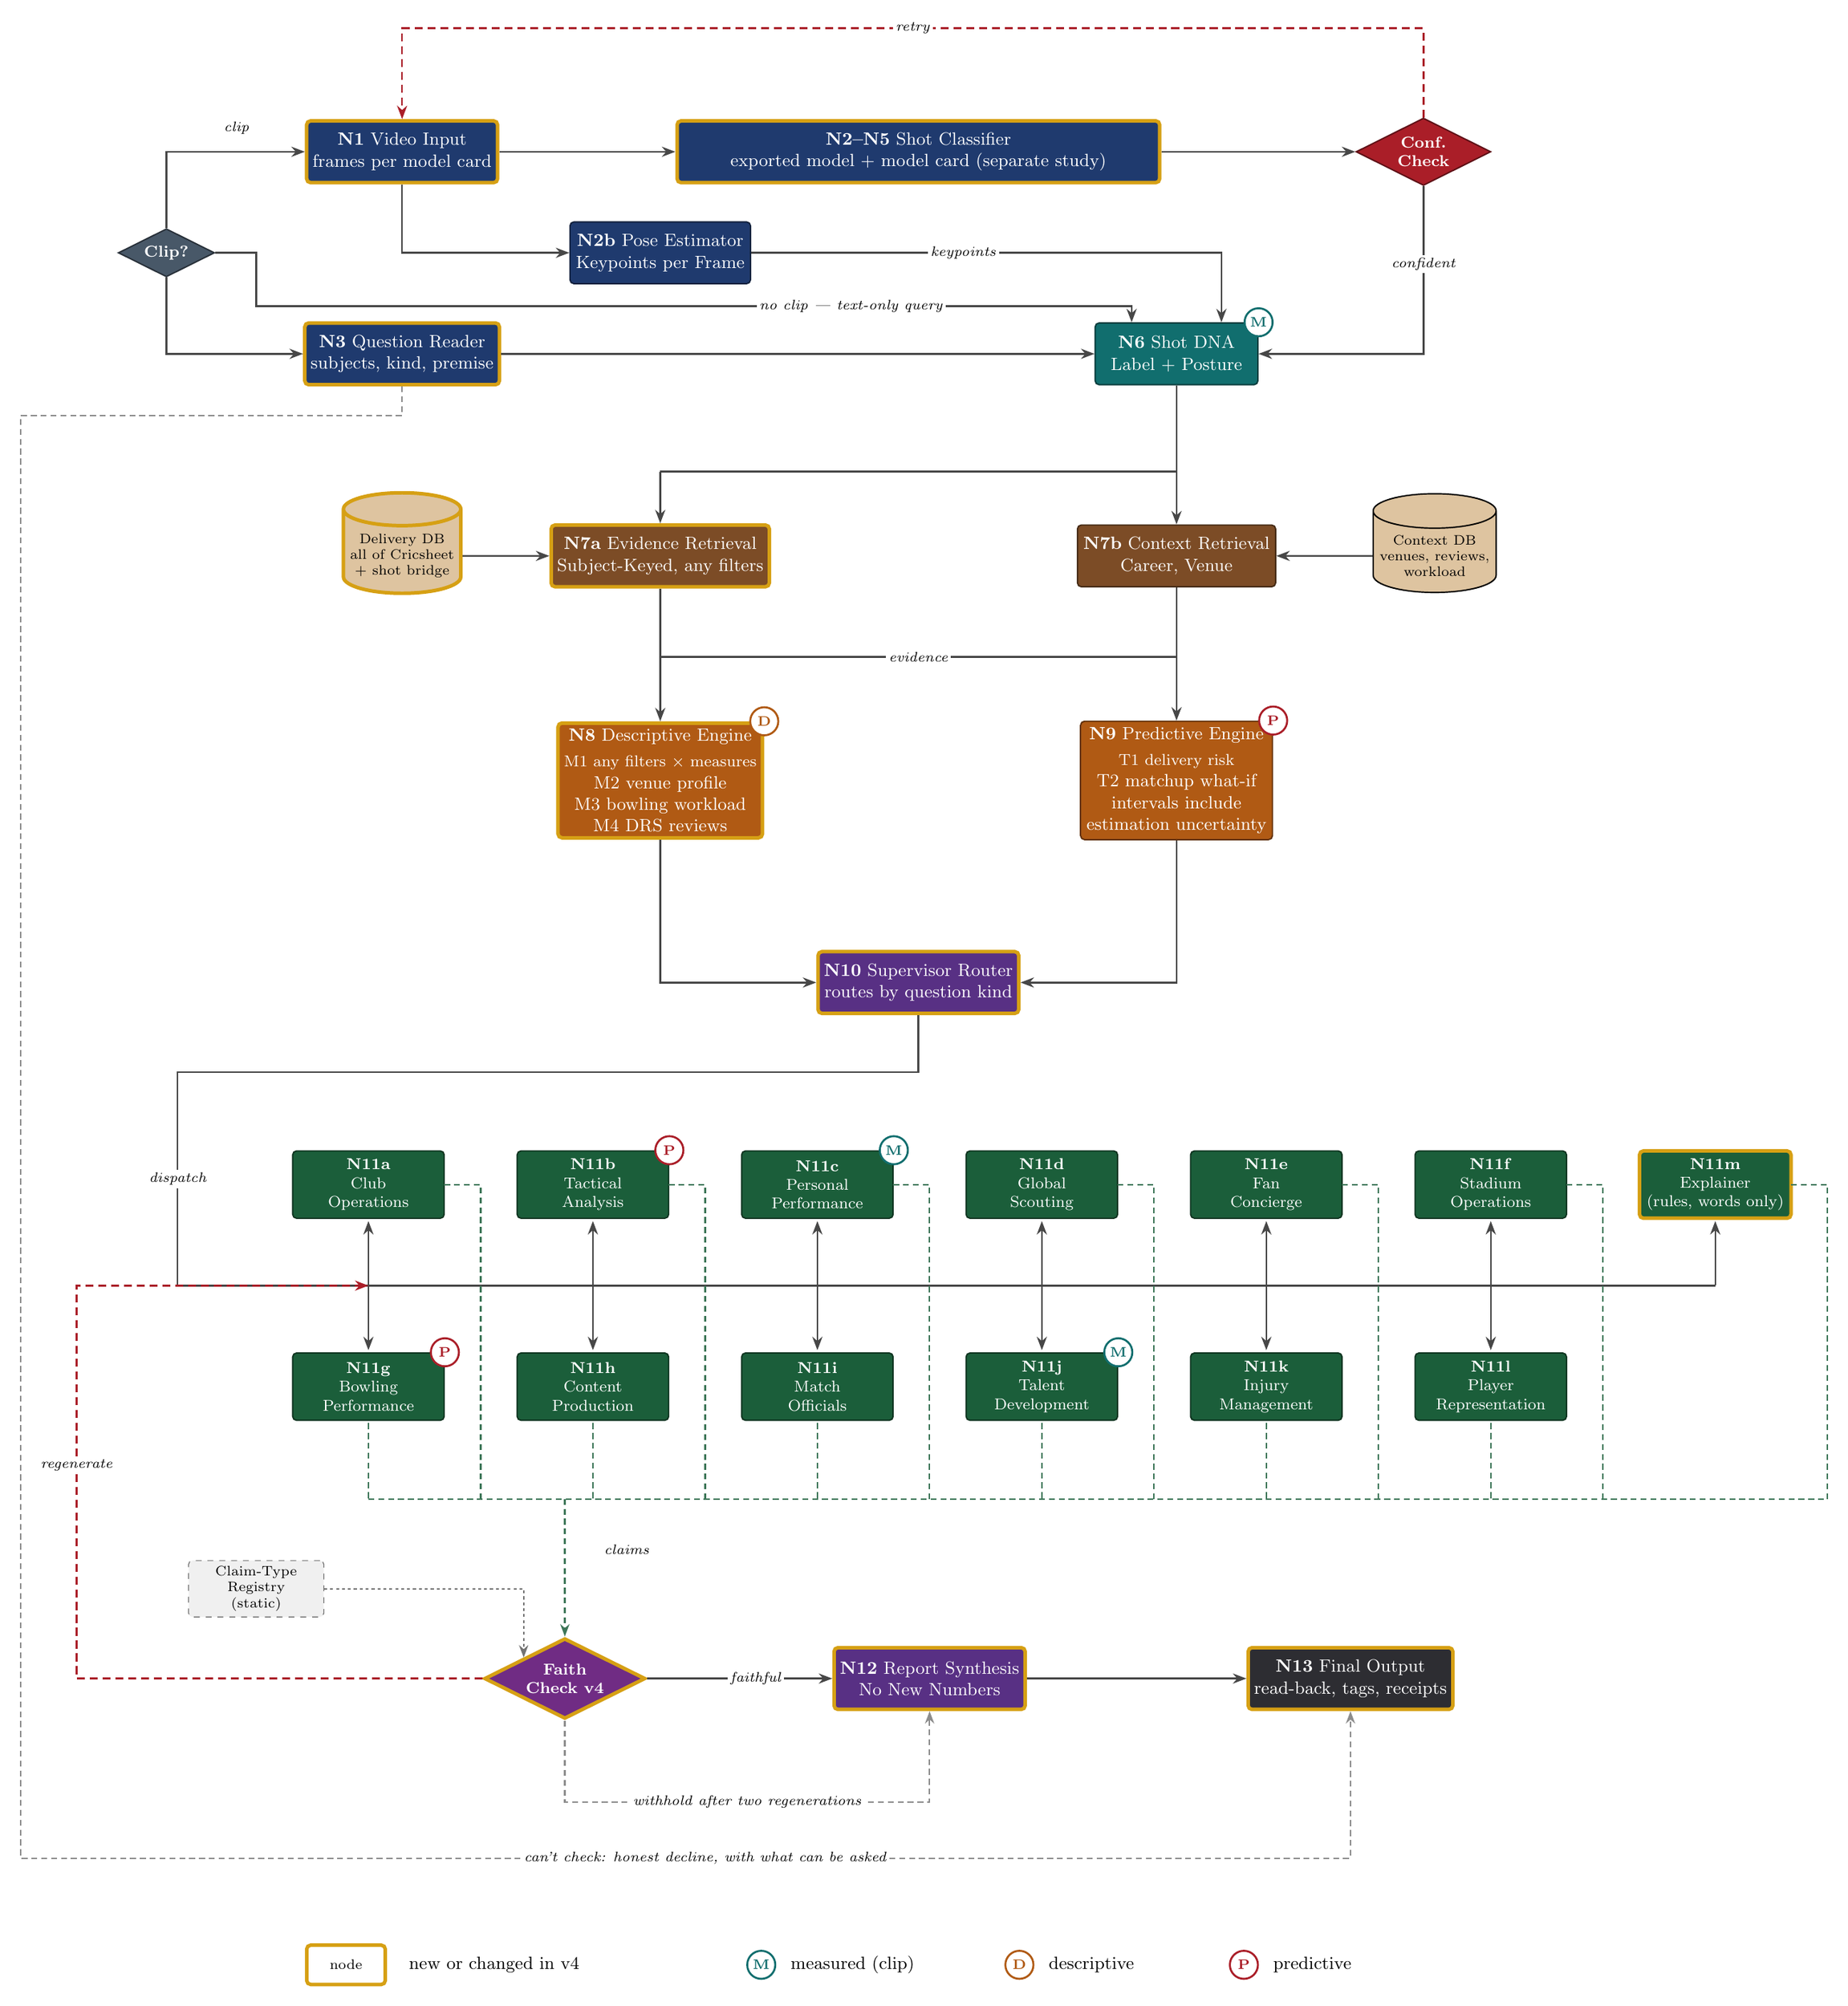
\begin{tikzpicture}

% ============================================ 0. entry branch
\node[entrygate] (entry) at (-2.6,-1.8) {Clip?};

% ============================================ A. perception (exported model)
\node[enc, v4] (n1)   at (1.6,0)    {\textbf{N1} Video Input\\frames per model card};
\node[enc, v4, minimum width=8.6cm] (clf) at (10.8,0)
  {\textbf{N2--N5} Shot Classifier\\exported model + model card (separate study)};
\node[confgate] (conf) at (19.8,0) {Conf.\\Check};

% ============================================ A'. pose branch
\node[enc] (n2b) at (6.2,-1.8) {\textbf{N2b} Pose Estimator\\Keypoints per Frame};

% ============================================ B. question reading + grounding
\node[enc, v4] (n3) at (1.6,-3.6)  {\textbf{N3} Question Reader\\subjects, kind, premise};
\node[fuse]    (n6) at (15.4,-3.6) {\textbf{N6} Shot DNA\\Label + Posture};

% ============================================ C. evidence and retrieval
\node[db, v4]  (db1) at (1.6,-7.2)  {Delivery DB\\all of Cricsheet\\+ shot bridge};
\node[ret, v4] (n7a) at (6.2,-7.2)  {\textbf{N7a} Evidence Retrieval\\Subject-Keyed, any filters};
\node[ret]     (n7b) at (15.4,-7.2) {\textbf{N7b} Context Retrieval\\Career, Venue};
\node[db]      (db2) at (20.0,-7.2) {Context DB\\venues, reviews,\\workload};

% ============================================ D. sanctioned engines
\node[svc, v4] (n8) at (6.2,-11.2)
  {\textbf{N8} Descriptive Engine\\[2pt]\footnotesize M1 any filters $\times$ measures\\
   M2 venue profile\\ M3 bowling workload\\ M4 DRS reviews};
\node[svc] (n9) at (15.4,-11.2)
  {\textbf{N9} Predictive Engine\\[2pt]\footnotesize T1 delivery risk\\
   T2 matchup what-if\\ intervals include\\ estimation uncertainty};

% ============================================ E. supervisor router
\node[route, v4] (n10) at (10.8,-14.8) {\textbf{N10} Supervisor Router\\routes by question kind};

% ============================================ F. agents and the Explainer
\node[agent] (ag1)  at (1,-18.4)  {\textbf{N11a}\\Club\\Operations};
\node[agent] (ag2)  at (5,-18.4)  {\textbf{N11b}\\Tactical\\Analysis};
\node[agent] (ag3)  at (9,-18.4)  {\textbf{N11c}\\Personal\\Performance};
\node[agent] (ag4)  at (13,-18.4) {\textbf{N11d}\\Global\\Scouting};
\node[agent] (ag5)  at (17,-18.4) {\textbf{N11e}\\Fan\\Concierge};
\node[agent] (ag6)  at (21,-18.4) {\textbf{N11f}\\Stadium\\Operations};
\node[agent, v4] (ag13) at (25,-18.4) {\textbf{N11m}\\Explainer\\(rules, words only)};

\node[agent] (ag7)  at (1,-22.0)  {\textbf{N11g}\\Bowling\\Performance};
\node[agent] (ag8)  at (5,-22.0)  {\textbf{N11h}\\Content\\Production};
\node[agent] (ag9)  at (9,-22.0)  {\textbf{N11i}\\Match\\Officials};
\node[agent] (ag10) at (13,-22.0) {\textbf{N11j}\\Talent\\Development};
\node[agent] (ag11) at (17,-22.0) {\textbf{N11k}\\Injury\\Management};
\node[agent] (ag12) at (21,-22.0) {\textbf{N11l}\\Player\\Representation};

% ============================================ G. verification and synthesis
\node[registry] (reg) at (-1.0,-25.6) {Claim-Type\\Registry\\(static)};
\node[faithgate, v4] (faith) at (4.5,-27.2) {Faith\\Check v4};
\node[route, v4] (n12) at (11,-27.2)   {\textbf{N12} Report Synthesis\\No New Numbers};
\node[outnode, v4] (n13) at (18.5,-27.2) {\textbf{N13} Final Output\\read-back, tags, receipts};

% ============================================ provenance badges
\node[badge=fuseteal]  at (n6.north east) {M};
\node[badge=svcorange] at (n8.north east) {D};
\node[badge=gatered]   at (n9.north east) {P};
\node[badge=gatered]   at (ag2.north east) {P};
\node[badge=gatered]   at (ag7.north east) {P};
\node[badge=fuseteal]  at (ag3.north east) {M};
\node[badge=fuseteal]  at (ag10.north east) {M};

% ==================================================================
%                              EDGES
% ==================================================================

% ---- entry branch; the text-only bypass runs in its own lane at y=-2.75
\draw[flow] (entry.north) -- (-2.6,0) -- (n1.west);
\node[elab] at (-1.35,0.42) {clip};
\draw[flow] (entry.south) -- (-2.6,-3.6) -- (n3.west);
\draw[flow] (entry.east) -- (-1.0,-1.8) -- (-1.0,-2.75) -- (14.6,-2.75)
            -- (14.6,0 |- n6.north);
\node[elab] at (9.6,-2.75) {no clip --- text-only query};

% ---- perception chain
\draw[flow] (n1) -- (clf);
\draw[flow] (clf) -- (conf);

% ---- pose branch: same frames, parallel to the classifier
\draw[flow] (n1.south) -- (1.6,-1.8) -- (n2b.west);
\draw[flow] (n2b.east) -- (16.2,-1.8) -- (16.2,0 |- n6.north);
\node[elab] at (11.6,-1.8) {keypoints};

% ---- retry loop
\draw[redloop] (conf.north) -- (19.8,2.2) -- (1.6,2.2) -- (n1.north);
\node[elab] at (10.7,2.2) {retry};

% ---- confident -> Shot DNA
\draw[flow] (conf.south) -- (19.8,-3.6) -- (n6.east);
\node[elab] at (19.8,-2.0) {confident};

% ---- question reader -> Shot DNA
\draw[flow] (n3.east) -- (n6.west);

% ---- honest decline: a can't-check question goes straight to the output
\draw[withhold] (n3.south) -- (1.6,-4.7) -- (-5.2,-4.7) -- (-5.2,-30.4)
                -- (18.5,-30.4) -- (n13.south);
\node[elab] at (7.0,-30.4) {can't check: honest decline, with what can be asked};

% ---- Shot DNA -> both retrievers
\draw[bus]  (n6.south) -- (15.4,-5.7);
\draw[bus]  (6.2,-5.7) -- (15.4,-5.7);
\draw[flow] (6.2,-5.7)  -- (n7a.north);
\draw[flow] (15.4,-5.7) -- (n7b.north);

% ---- databases -> retrievers
\draw[flow] (db1) -- (n7a);
\draw[flow] (db2) -- (n7b);

% ---- retrievers -> engines
\draw[bus]  (n7a.south) -- (6.2,-9.0);
\draw[bus]  (n7b.south) -- (15.4,-9.0);
\draw[bus]  (6.2,-9.0) -- (15.4,-9.0);
\draw[flow] (6.2,-9.0)  -- (n8.north);
\draw[flow] (15.4,-9.0) -- (n9.north);
\node[elab] at (10.8,-9.0) {evidence};

% ---- engines -> router
\draw[flow] (n8.south) -- (6.2,-14.8)  -- (n10.west);
\draw[flow] (n9.south) -- (15.4,-14.8) -- (n10.east);

% ---- router -> dispatch bus
\draw[bus] (n10.south) -- (10.8,-16.4) -- (-2.4,-16.4) -- (-2.4,-20.2) -- (1,-20.2);
\draw[bus] (1,-20.2) -- (25,-20.2);
\node[elab] at (-2.4,-18.3) {dispatch};

% ---- dispatch bus -> each agent
\draw[flow] (1,-20.2)  -- (1,-19.05);
\draw[flow] (5,-20.2)  -- (5,-19.05);
\draw[flow] (9,-20.2)  -- (9,-19.05);
\draw[flow] (13,-20.2) -- (13,-19.05);
\draw[flow] (17,-20.2) -- (17,-19.05);
\draw[flow] (21,-20.2) -- (21,-19.05);
\draw[flow] (25,-20.2) -- (25,-19.05);

\draw[flow] (1,-20.2)  -- (1,-21.35);
\draw[flow] (5,-20.2)  -- (5,-21.35);
\draw[flow] (9,-20.2)  -- (9,-21.35);
\draw[flow] (13,-20.2) -- (13,-21.35);
\draw[flow] (17,-20.2) -- (17,-21.35);
\draw[flow] (21,-20.2) -- (21,-21.35);

% ---- collection bus (green dashed) below row 2
\draw[ybus] (1,-24.0) -- (27,-24.0);

\draw[ybus] (1,-22.65)  -- (1,-24.0);
\draw[ybus] (5,-22.65)  -- (5,-24.0);
\draw[ybus] (9,-22.65)  -- (9,-24.0);
\draw[ybus] (13,-22.65) -- (13,-24.0);
\draw[ybus] (17,-22.65) -- (17,-24.0);
\draw[ybus] (21,-22.65) -- (21,-24.0);

\draw[ybus] (2.35,-18.4)  -- (3,-18.4)  -- (3,-24.0);
\draw[ybus] (6.35,-18.4)  -- (7,-18.4)  -- (7,-24.0);
\draw[ybus] (10.35,-18.4) -- (11,-18.4) -- (11,-24.0);
\draw[ybus] (14.35,-18.4) -- (15,-18.4) -- (15,-24.0);
\draw[ybus] (18.35,-18.4) -- (19,-18.4) -- (19,-24.0);
\draw[ybus] (22.35,-18.4) -- (23,-18.4) -- (23,-24.0);
\draw[ybus] (26.35,-18.4) -- (27,-18.4) -- (27,-24.0);

% ---- claims -> Faith Check; the registry defines what C1 accepts
\draw[yield] (4.5,-24.0) -- (faith.north);
\node[elab] at (5.6,-24.9) {claims};
\draw[static] (reg.east) -- (reg.east -| faith.north west) -- (faith.north west);

% ---- faith check -> synthesis -> output
\draw[flow] (faith.east) -- (n12.west);
\node[elab] at (7.9,-27.2) {faithful};
\draw[flow] (n12.east) -- (n13.west);

% ---- regenerate loop: back to the dispatch bus, failing agents only
\draw[redloop] (faith.west) -- (-4.2,-27.2) -- (-4.2,-20.2) -- (1,-20.2);
\node[elab] at (-4.2,-23.4) {regenerate};

% ---- withhold path: budget spent, the finding is listed but not used
\draw[withhold] (faith.south) -- (4.5,-29.4) -- (11,-29.4) -- (n12.south);
\node[elab] at (7.75,-29.4) {withhold after two regenerations};

% ============================================ legend
\node[draw=newgold, line width=1.8pt, rounded corners=2pt, fill=white,
      minimum width=1.4cm, minimum height=0.7cm, font=\scriptsize] at (0.6,-32.3) {node};
\node[anchor=west, font=\small] at (1.6,-32.3) {new or changed in v4};
\node[badge=fuseteal]  at (8.0,-32.3) {M};
\node[anchor=west, font=\small] at (8.4,-32.3) {measured (clip)};
\node[badge=svcorange] at (12.6,-32.3) {D};
\node[anchor=west, font=\small] at (13.0,-32.3) {descriptive};
\node[badge=gatered]   at (16.6,-32.3) {P};
\node[anchor=west, font=\small] at (17.0,-32.3) {predictive};

\end{tikzpicture}}

\captionof{figure}{CricketMind LangGraph architecture, Version~4. Gold outlines
mark nodes that are new or changed since v3. Badges give the provenance class a
node produces or an agent may cite: M for measured from the clip, D for
descriptive (counted from history), P for predictive (simulated). N3 gives every
question one of five kinds (Table~\ref{tab:kinds}). A question nothing can check
goes straight to the output with an honest decline; for a rules question the
evidence and engine nodes pass the state through unchanged and N10 sends it to
the Explainer, N11m. Agents emit claim tuples rather than numbers; the Faith
Check re-queries the engines for each tuple, keeps the receipt of that
re-query, and runs checks C1--C7 (Figure~\ref{fig:faith-v4}) against the static
claim-type registry. Failing agents are regenerated with the reasons, at most
twice, after which the finding is withheld and listed in the report. The
classifier N2--N5 is one exported model from a separate study, and N1 picks
frames exactly as its model card states. Data sources and the offline pipeline
are shown in Figure~\ref{fig:offline}.}
\label{fig:arch-v4}
\end{keep}

% =====================================================================
\clearpage
\section{Answering Any Question Honestly}
\label{sec:any}

N3 keeps the structured parse of Version~3 and also gives every question one of
five kinds (Table~\ref{tab:kinds}). The kind decides the path, and the path
decides what kind of answer is possible.

\begin{table}[htbp]
\centering
\footnotesize
\renewcommand{\arraystretch}{1.25}
\begin{tabular}{@{}>{\raggedright\arraybackslash}p{1.8cm}
                  >{\raggedright\arraybackslash}p{4.6cm}
                  >{\raggedright\arraybackslash}p{2.8cm}
                  >{\raggedright\arraybackslash}p{5.6cm}@{}}
\toprule
\textbf{Kind} & \textbf{Example} & \textbf{Path} & \textbf{Answer} \\
\midrule
Stats & ``Kohli's batting average against Australia since 2020?'' & N7a, N8 M1 & checked facts, tagged D \\
Prediction & ``The chance Kohli is out within six short balls of pace in the powerplay?'' & N7a, N9 & checked, with its interval; the wording must fit its band (C4) \\
Video & ``Is this a cover drive? Is his weight forward?'' & N1--N5, N2b, N6 & the label with its confidence; measured posture, tagged M \\
Rules & ``What is LBW?'' & the Explainer, N11m & words only, labelled ``general explanation, not checked against data'' \\
Can't check & ``Is Kohli injured?'' & none & ``I can't check that'', and what can be asked instead \\
\bottomrule
\end{tabular}
\caption{The five kinds of question. Every answer starts with a
read-back of how the question was understood.}
\label{tab:kinds}
\end{table}

\paragraph{The read-back.} Every answer begins ``I read this as: \ldots'', listing
the parsed player, measure, filters and scope, for example ``I read this as:
V Kohli; batting average; against Australia; since 2020; all formats.'' A
misreading then shows on the screen instead of silently answering a different
question.

\paragraph{Filters times measures.} In Version~3 each claim type was, in effect,
one fixed question. In Version~4, N8 M1 computes any registered \emph{measure}
(batting: runs, strike rate, average, dismissal rate, boundary and dot-ball
share; bowling: wickets, economy, bowling strike rate) under any combination of
supported \emph{filters} (player, bowler, opposition, venue, season, format,
innings, phase, bowler type, batting hand). The registry lists measures, not
questions, so a small registry answers a very large number of questions, each
computed by the engine and checked by C2. A new measure is one registry row, one
engine function and one line of renderer words. Language-model-written SQL is
deliberately not used: on cricket questions most such SQL executes while little
of it returns the right answer \cite{cricbench}, and nothing would check it.

\paragraph{Paraphrases.} Different wordings of one question should parse to the
same subjects and measure, and so reach the same engine query and the same
verified answer. This is tested directly: the locked exam asks questions in
several wordings (Section~\ref{sec:eval}).

\paragraph{The Explainer, N11m.} Rules and general questions go to a new node
that answers in words only. Its answer is labelled ``general explanation, not
checked against data''; C5 still forbids digits, apart from a small allowlist
(``T20'', ``U-19''); and it may not name players, since any statement about a
player needs data. A checked rules source, such as the MCC Laws of Cricket, is
future work.

\paragraph{The honest decline.} If no engine could answer (injuries, salaries,
private medical or contract data), N3 marks the question \emph{can't check} and
the output says so, with examples of what can be asked instead. No agent is
woken, and nothing is invented.

% =====================================================================
\section{Node-by-Node Changes}

\subsection{Perception through an Exported Model: N1--N5}

In Version~3, N2, N4 and N5 named an EfficientNetV2-S frame encoder, a temporal
transformer and a fifteen-class head. The classifier is now built in a separate
study, CricShot, and reaches CricketMind as one exported model with a model card
that states exactly what input it expects. CricketMind never imports CricShot
code; the choice of backbone and its accuracy belong to that study.

Frame selection is part of this contract. CricShot's preprocessing drops repeated
frames (some clips carry copies inserted by frame-rate conversion), finds the
batter, keeps the camera shot with the most detections, crops to it, and only
then takes evenly spaced frames from what remains. Fifteen evenly spaced frames
from the raw clip would feed the model inputs it never saw in training, and no
error would be raised. N1 therefore follows the model card, and a parity test
compares CricketMind's frames and crops with CricShot's on a fixed set of clips:
frame numbers exactly, pixels within a tolerance. The confidence check and its
two retries are unchanged.

\subsection{N2b Pose Estimator}

Unchanged from Version~3. A pose model \cite{yolo} extracts seventeen body
keypoints per frame on the same frames, and three posture metrics are computed:
weight transfer, stride length, and head over front knee, each scaled so that it
does not depend on camera distance. Posture has no ground truth, so each metric
is validated by how well it separates shots played mainly off the front foot from
shots played mainly off the back foot (ROC-AUC on the CricShot10k test split,
threshold $0.75$, a design parameter). A metric that fails leaves the registry.
The test uses dataset labels, not the classifier, and reports no classifier
accuracy.

\subsection{N3 Question Reader}

N3 keeps Version~3's structured parse under a fixed schema (batter, bowlers,
shots, phase, bowler type, venue, format, and an optional scenario), with every
name resolved against the player register and an unknown player reported as
such. It adds three outputs: the \emph{kind} of question (Section~\ref{sec:any});
the \emph{read-back}; and any \emph{premise}, a judgment the question takes for
granted. ``Why is Kohli bad against spin?'' presupposes that he is worse than
average against spin. A marked premise becomes a comparison the agents must cite
and C7 must check (Section~\ref{sec:faith}). Text inside a question is only ever
read as a question, never as an instruction to the system.

\subsection{N6 Shot DNA}

Unchanged. N6 fuses the accepted shot label, the measured posture (provenance M,
video path only, invariant I5) and the parsed subjects into one record.
Downstream nodes never see a pixel.

\subsection{Evidence Layer and Retrieval}

\begin{table}[htbp]
\centering
\footnotesize
\renewcommand{\arraystretch}{1.25}
\begin{tabular}{@{}>{\raggedright\arraybackslash}p{3.3cm}
                  >{\raggedright\arraybackslash}p{4.5cm}
                  >{\raggedright\arraybackslash}p{3.0cm}
                  >{\raggedright\arraybackslash}p{4.2cm}@{}}
\toprule
\textbf{Source} & \textbf{Provides} & \textbf{Does not provide} & \textbf{Access and caveats} \\
\midrule
CricShot10k \cite{cricshot10k} & 15-class batting-shot clips & identity, outcome & held locally \\
Cricsheet \cite{cricsheet}, every competition, men's and women's & every delivery: batter, bowler, runs, extras, wicket, venue, date; DRS reviews & shot type, line and length, bowler type & free with attribution; the snapshot's date and checksum are recorded; review data has needed corrections \cite{cricsheetreview} \\
Player register with Cricinfo attributes \cite{cricketdata} & batting hand, bowling type & --- & identifiers link the two; check terms of use \\
Commentary corpus & text that names the stroke played & shot labels; match and ball keys unverified & no clean, labelled public corpus was found; must be licensed \\
Open football event data \cite{statsbomb} & every pass, shot and tackle of the matches covered & --- & case study only (Section~\ref{sec:general}); check the licence; pin a snapshot \\
Injury, replay, sponsorship, eligibility, salary records & nothing public & --- & questions about them get an honest decline \\
\bottomrule
\end{tabular}
\caption{Evidence sources.}
\label{tab:data}
\end{table}

\begin{figure}[htbp]
\centering
\resizebox{\textwidth}{!}{%
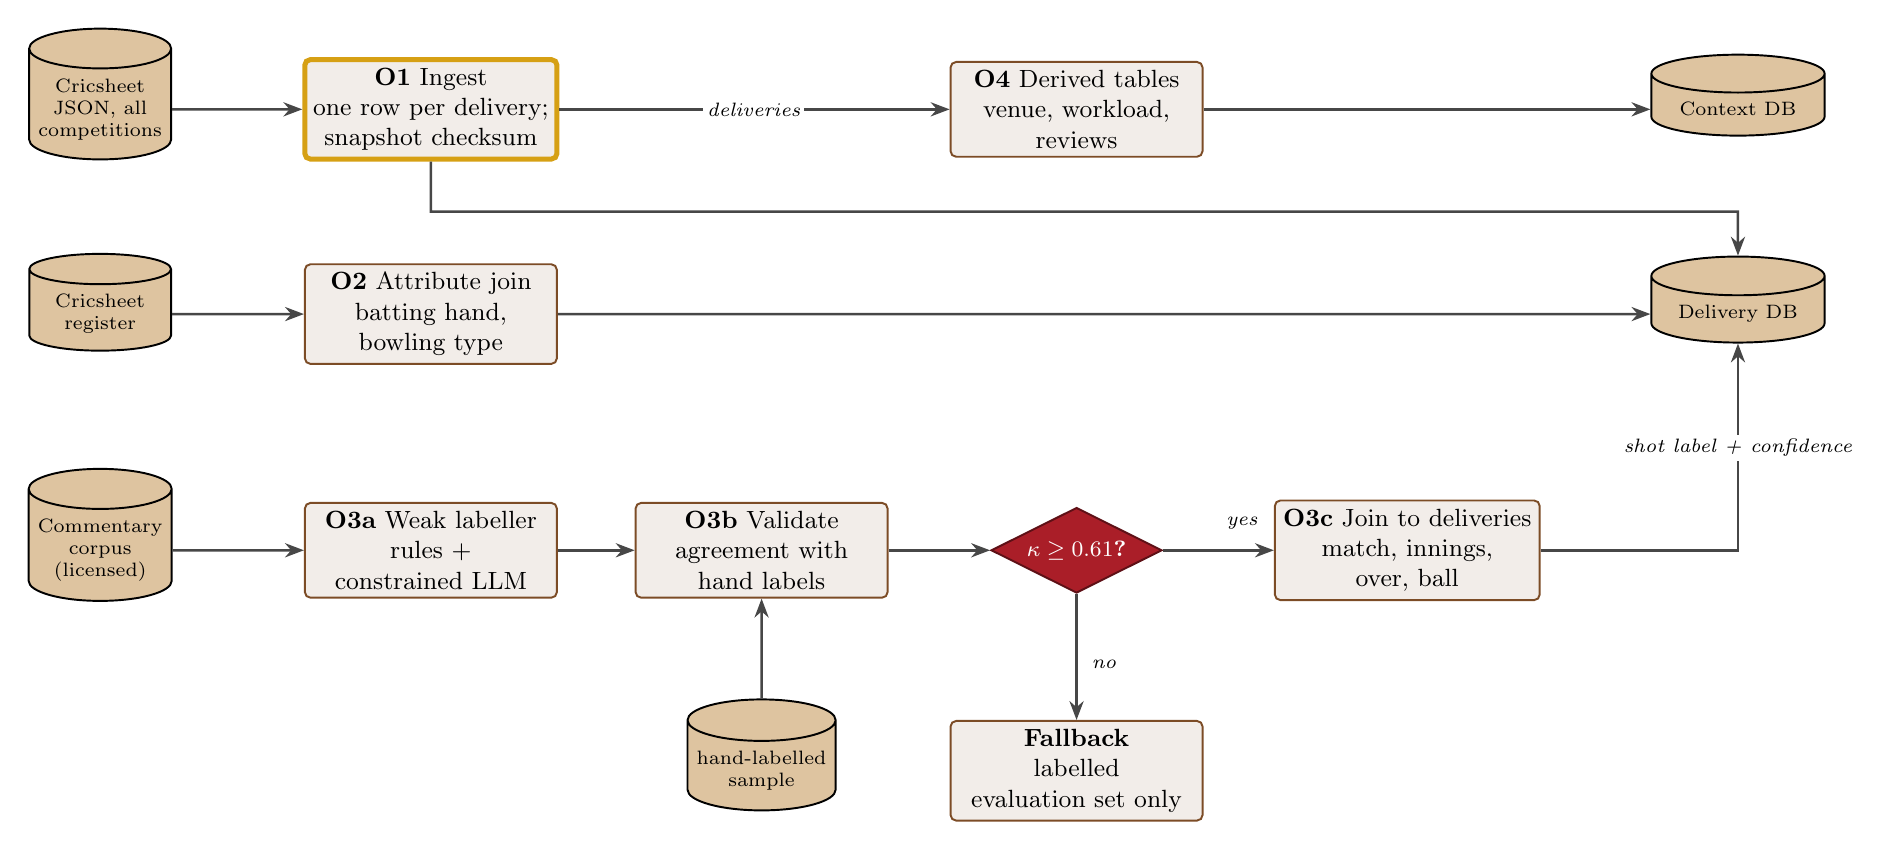
\begin{tikzpicture}

% ---- sources
\node[db] (s1) at (0,0)    {Cricsheet\\JSON, all\\competitions};
\node[db] (s2) at (0,-2.6) {Cricsheet\\register};
\node[db] (s3) at (0,-5.6) {Commentary\\corpus\\(licensed)};

% ---- processing
\node[off, v4] (o1) at (4.2,0)    {\textbf{O1} Ingest\\one row per delivery;\\snapshot checksum};
\node[off] (o4)  at (12.4,0)   {\textbf{O4} Derived tables\\venue, workload,\\reviews};
\node[off] (o2)  at (4.2,-2.6) {\textbf{O2} Attribute join\\batting hand,\\bowling type};
\node[off] (o3a) at (4.2,-5.6) {\textbf{O3a} Weak labeller\\rules +\\constrained LLM};
\node[off] (o3b) at (8.4,-5.6) {\textbf{O3b} Validate\\agreement with\\hand labels};
\node[confgate] (kg) at (12.4,-5.6) {$\kappa \geq 0.61$?};
\node[off] (o3c) at (16.6,-5.6) {\textbf{O3c} Join to deliveries\\match, innings,\\over, ball};
\node[db]  (hl)  at (8.4,-8.4) {hand-labelled\\sample};
\node[off] (fb)  at (12.4,-8.4) {\textbf{Fallback}\\labelled\\evaluation set only};

% ---- outputs
\node[db, minimum width=2.2cm] (cdb) at (20.8,0)    {Context DB};
\node[db, minimum width=2.2cm] (ddb) at (20.8,-2.6) {Delivery DB};

% ---- edges
\draw[flow] (s1) -- (o1);
\draw[flow] (s2) -- (o2);
\draw[flow] (s3) -- (o3a);
\draw[flow] (o1) -- (o4);
\node[elab] at (8.3,0) {deliveries};
\draw[flow] (o4) -- (cdb);
\draw[flow] (o1.south) -- (4.2,-1.3) -- (20.8,-1.3) -- (ddb.north);
\draw[flow] (o2) -- (ddb);
\draw[flow] (o3a) -- (o3b);
\draw[flow] (hl) -- (o3b);
\draw[flow] (o3b) -- (kg);
\draw[flow] (kg) -- (o3c);
\node[elab] at (14.5,-5.25) {yes};
\draw[flow] (kg) -- (fb);
\node[elab] at (12.75,-7.05) {no};
\draw[flow] (o3c.east) -- (20.8,-5.6) -- (ddb.south);
\node[elab] at (20.8,-4.3) {shot label + confidence};

\end{tikzpicture}}
\caption{Offline evidence pipeline. Nothing here runs at query time.
The commentary bridge (O3) is accepted only if its labels agree substantially
with a hand-labelled sample; otherwise shot-keyed statistics are restricted to a
hand-labelled evaluation set.}
\label{fig:offline}
\end{figure}

\paragraph{O1, O2, O4: ball-by-ball evidence.} O1 flattens every Cricsheet
competition into one row per delivery and records the snapshot's date and
checksum, which every receipt names. O2 attaches batting hand and bowling type
through the player register, so that filters such as ``against pace'' have a
source. O4 derives the tables the N8 modules read: venue aggregates, balls bowled
per bowler per date, and the DRS reviews attached to deliveries.

\paragraph{O3: the commentary-to-shot bridge.} Unchanged from Version~3.
Ball-by-ball commentary names the stroke (``drives through cover''), but no
labelled dataset pairs commentary with the fifteen CricShot10k classes. O3a
labels each line weakly \cite{snorkel}: keyword rules first, then, for lines the
rules cannot resolve, a language model constrained to the fifteen classes or
\emph{none}. O3b measures agreement with a stratified hand-labelled sample of
about 500 lines by Cohen's $\kappa$ \cite{cohen} and per-class F1; the bridge is
accepted at $\kappa \geq 0.61$, ``substantial'' agreement \cite{landis}. O3c
joins labels to deliveries by match, innings, over and ball; each label keeps its
confidence and origin. The language model produces categories that are validated
before use, never a number an agent can cite, so invariant I1 is untouched.

\paragraph{N7a and N7b.} N7a filters by any combination of the supported filters
and returns the matching deliveries with their count. A shot filter applies only
to deliveries the bridge labelled. N7b retrieves career and venue context as
before.

\subsection{N8 Descriptive Engine}

N8 stays deterministic aggregation over a pinned data snapshot: every output can
be recomputed by hand, and every receipt reproduces it.

\begin{description}[leftmargin=1.2em,style=nextline,itemsep=2pt]
\item[M1 --- delivery statistics, any filters $\times$ measures.] The measures
  and filters of Section~\ref{sec:any}, with sample sizes; differences between
  two subjects with a bootstrap 95\% interval (used by C4); and
  \texttt{sr\_vs\_average}, a player's strike rate against the average batter
  under the same filters, with a bootstrap interval (used by C7).
\item[M2 --- venue profile] (backs N11f). Average first-innings score, share of
  matches won chasing, and the share of wickets taken by pace and by spin.
\item[M3 --- bowling workload] (backs N11k). Balls bowled in the last 7 and 28
  days and their ratio. Workload spikes were associated with roughly double the
  injury risk in the following week in elite fast bowlers \cite{hulin}, but the
  ratio's validity is disputed \cite{impellizzeri}, and match data omits training
  loads. M3 therefore emits a \emph{monitoring flag}, never an injury
  probability.
\item[M4 --- DRS reviews] (backs N11i). Review counts and overturn rates by team
  and by dismissal type.
\end{description}

\subsection{N9 Predictive Engine and Honest Uncertainty}
\label{sec:uncert}

\paragraph{T1 and T2.} Unchanged from Version~3. Tier~1 answers the delivery
question (``six short balls: what is the chance of a wicket?''). Tier~2 answers
matchup counterfactuals (``what if this bowler bowled the over instead of that
one?''), estimated from head-to-head rates shrunk toward population rates
\cite{efron}. A counterfactual is always reported as a difference against a
baseline, with an interval; if the interval contains zero, the output is
\emph{no detectable difference}.

\paragraph{Two kinds of uncertainty.} v2's interval measured only Monte Carlo
error, which shrinks as trials increase; it omitted estimation uncertainty,
which shrinks only with more data. On the synthetic corpus (illustrative only),
the batter's pull has 4 dismissals in 50 balls:

\begin{center}
\small
\begin{tabular}{@{}lcc@{}}
\toprule
& \textbf{P(out within 6 balls)} & \textbf{95\% interval} \\
\midrule
v2: Monte Carlo error only (20,000 trials) & 0.394 & [0.387, 0.400] \\
since v3: estimation uncertainty propagated & 0.405 (median) & [0.155, 0.697] \\
\bottomrule
\end{tabular}
\end{center}

\noindent The second row draws the per-ball rate from a Beta posterior (Jeffreys
prior) and pushes each draw through the simulation. The honest interval is about
twenty times wider, and it spans three wording bands of Table~\ref{tab:lexicon}.

\paragraph{Calibration.} T1 and T2 are calibrated on a held-out season:
reliability diagrams and the Brier score \cite{brier}.

\subsection{N10 Supervisor Router}

The router keeps Version~3's evidence summary, its capability filter, the cap of
four active agents and the default pair. It now also routes by kind: stats,
prediction and video questions go to the stakeholder agents, and rules questions
go to the Explainer, which counts as one of the four.

\subsection{The Agents}

\begin{table}[H]
\centering
\footnotesize
\renewcommand{\arraystretch}{1.25}
\begin{tabular}{@{}>{\raggedright\arraybackslash}p{3.0cm}
                  >{\raggedright\arraybackslash}p{3.4cm}
                  >{\raggedright\arraybackslash}p{7.4cm}
                  >{\raggedright\arraybackslash}p{1.0cm}@{}}
\toprule
\textbf{Stakeholder} & \textbf{Agent} & \textbf{Claim types it may assert} & \textbf{Prov.} \\
\midrule
Franchises / Boards & Club Operations (N11a) & strike rate, dismissal rate, sample size; venue profile & D \\
Coaches & Tactical Analysis (N11b) & strike and dismissal rates; P(dismissal within $k$); matchup difference & D, P \\
Players & Personal Performance (N11c) & strike rates; posture metrics & D, M \\
Scouts & Global Scouting (N11d) & strike rate, career strike rate, league benchmark & D \\
Fans & Fan Concierge (N11e) & venue strike rate, strike rate, recent form & D \\
Stadiums / curators & Stadium Operations (N11f) & first-innings average, chasing share, pace and spin wicket share & D \\
Bowlers / bowling coaches & Bowling Performance (N11g) & economy and dismissal rate by phase and batting hand; matchup difference & D, P \\
Broadcasters / sponsors & Content Production (N11h) & strike rates; boundary counts as a visibility proxy & D \\
Governing bodies / umpires & Match Officials (N11i) & review counts, overturn rate by team and dismissal type & D \\
Academies & Talent Development (N11j) & strike rates; posture metrics & D, M \\
Medical teams & Injury Management (N11k) & balls bowled (7 and 28 days), workload ratio flag & D \\
Player agents & Player Representation (N11l) & strike rate, career strike rate & D \\
Anyone asking about rules & \textbf{Explainer (N11m)} & none: words only, labelled, no digits, no player names & --- \\
\bottomrule
\end{tabular}
\caption{The Version~4 roster: Version~3's twelve agents and the
Explainer. Every claim type in the third column is a registry entry backed by an
engine metric (invariant I2), and every agent's tone words must now be backed by
a checked comparison (C7).}
\label{tab:roster}
\end{table}

% =====================================================================
\section{The Claim Contract}
\label{sec:claims}

An agent finding is a list of claims and a prose template. The claim is the unit
of verification:

\medskip
{\footnotesize
\begin{verbatim}
{"id": "c1", "kind": "descriptive", "metric": "strike_rate", "engine": "N8.M1",
 "subject": {"player": "V Kohli", "shot": "Cover Drive", "phase": "powerplay",
             "bowler_type": "pace"},
 "value": 142.0, "n": 50}
{"id": "c2", "kind": "predictive", "metric": "p_dismissal_within_k", "engine": "N9.T1",
 "subject": {"player": "V Kohli", "shot": "Pull", "phase": "powerplay",
             "bowler_type": "pace", "k": 6},
 "value": 0.405, "interval": [0.155, 0.697]}

template: "Against pace in the powerplay, Kohli's cover drive returns {c1}.
           Six short balls carry {c2} of a dismissal."
rendered: "Against pace in the powerplay, Kohli's cover drive returns a strike
           rate of 142.0 [D, 50 balls]. Six short balls carry a 41% chance
           [P, range 16% to 70%] of a dismissal."
\end{verbatim}}
\medskip

\noindent The values are the synthetic examples of Section~\ref{sec:uncert}, and
the rendered line is the output of the built renderer.

\paragraph{Claims check themselves (built).} A claim refuses to exist if it
breaks one of four rules: its identifier is \texttt{c} followed by digits, so
templates can reference it; a descriptive claim carries its sample size,
$n \geq 1$; a predictive claim carries a 95\% interval that contains its value;
a measured claim names its clip (I5). The wording band of a predictive claim is
not stored, as Version~3's example did, but computed from the value when C4 needs
it, so the two can never disagree. Claims and findings are immutable once made,
and a finding keeps its claims in an immutable sequence, so nothing can be added
after the check.

\paragraph{The renderer (built).} A deterministic renderer replaces each
reference with words, the verified value and a tag: \texttt{[D, 50 balls]},
\texttt{[P, range 16\% to 70\%]}, \texttt{[M, clip vid1\_0]}. The agent never
types a digit (I3). Displayed numbers round exact halves up, in decimal
arithmetic on the number's shortest written form: 0.405 shows as 41\%, 0.155 as
16\% and 0.145 as 15\%. Python's default formatting gives 40\%, 16\% and 14\% for
the same values, because it rounds an exact half to the even neighbour and
because $0.145 \times 100$ falls just below 14.5 in binary floating point; a
reader comparing the report with the engine would see unexplained one-point
differences.

\paragraph{Subjects: one shared base.} The checks, the claims and the renderer
only ever see a \texttt{Subject}; each sport defines its own fields.

\medskip
{\footnotesize
\begin{verbatim}
@dataclass(frozen=True, kw_only=True)
class Subject:                      # the checks only ever see this
    pass

@dataclass(frozen=True, kw_only=True)
class CricketSubject(Subject):
    player: str | None = None
    shot: str | None = None
    phase: str | None = None
    bowler_type: str | None = None
    # bowler, other_bowler, other_shot, venue, match_format,
    # team, dismissal_type, date, k
\end{verbatim}}
\medskip

\noindent Fields are keyword-only, so \texttt{CricketSubject("Pull", "V Kohli")},
which would silently swap player and shot, is refused; subjects are frozen, so a
checked claim's subject cannot change. A football subject is another subclass,
and nothing in the checks changes (Section~\ref{sec:general}).

\paragraph{Receipts.} When C2 re-queries the named engine for a claim's subject,
the gate keeps that query as the claim's receipt: the checksum of the pinned data
snapshot, the exact engine query and the engine's version. N13 shows the receipt
with the number, and a receipt checker re-runs any receipt and confirms the
value. Receipts come from the gate's own re-query, never from the agent.

\paragraph{The claim-type registry.} Table~\ref{tab:registry} shows the registry
at its first build. It is built with the graph, and two things are checked then:
every claim type an agent declares exists, and every registry entry resolves to
an engine metric. A template that asserts ``the surface is holding pace'' with no
venue metric behind it is therefore not a runtime failure but a build failure.
The measures of Section~\ref{sec:any} join it later, one row each.

\begin{table}[htbp]
\centering
\footnotesize
\renewcommand{\arraystretch}{1.2}
\begin{tabular}{@{}>{\raggedright\arraybackslash}p{4.3cm}
                  >{\raggedright\arraybackslash}p{1.0cm}
                  >{\raggedright\arraybackslash}p{1.3cm}
                  >{\raggedright\arraybackslash}p{4.2cm}
                  >{\raggedright\arraybackslash}p{4.1cm}@{}}
\toprule
\textbf{Claim type} & \textbf{Prov.} & \textbf{Source} & \textbf{Required subject keys} & \textbf{Checks} \\
\midrule
\texttt{strike\_rate} & D & N8.M1 & player; other filters optional & C2 exact; C3 floor \\
\texttt{dismissal\_rate} & D & N8.M1 & as above & C2; C3 \\
\texttt{sr\_difference} & D & N8.M1 & player, two shots & C2; C4 zero-crossing; backs C7 \\
\texttt{sr\_vs\_average} & D & N8.M1 & player; compared with the average batter under the same filters & C2; C3; backs C7 \\
\texttt{venue\_first\_innings\_avg} & D & N8.M2 & venue, format & C2; C3 (matches) \\
\texttt{workload\_ratio\_flag} & D & N8.M3 & bowler, date & C2; wording: flag only \\
\texttt{review\_overturn\_rate} & D & N8.M4 & team or dismissal type & C2; C3 \\
\texttt{weight\_transfer} & M & N6 & a clip & C2; video path only \\
\texttt{p\_dismissal\_within\_k} & P & N9.T1 & player, shot, phase, bowler type, $k$ & C2 with interval; C4 band \\
\texttt{matchup\_difference} & P & N9.T2 & batter, two bowlers, phase, $k$ & C2 with interval; C4 zero-crossing \\
\bottomrule
\end{tabular}
\caption{The claim-type registry at its first build: the nine types of
Version~3 and \texttt{sr\_vs\_average}.}
\label{tab:registry}
\end{table}

% =====================================================================
\section{Faith Check v4}
\label{sec:faith}

\begin{figure}[H]
\centering
\resizebox{\textwidth}{!}{%
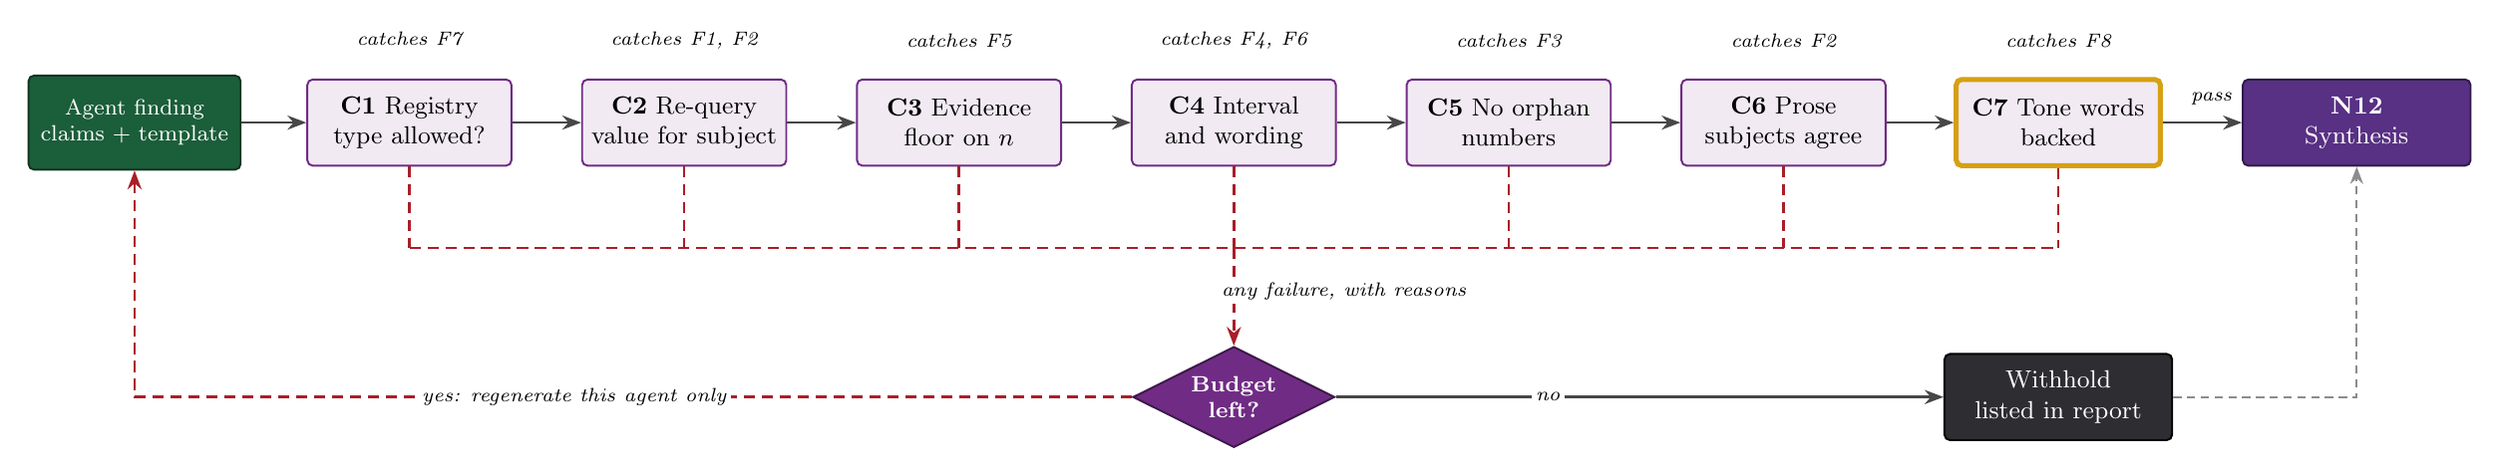
\begin{tikzpicture}

\node[agent] (fd) at (0,0)    {Agent finding\\claims + template};
\node[chk] (c1) at (3.5,0)  {\textbf{C1} Registry\\type allowed?};
\node[chk] (c2) at (7.0,0)  {\textbf{C2} Re-query\\value for subject};
\node[chk] (c3) at (10.5,0) {\textbf{C3} Evidence\\floor on $n$};
\node[chk] (c4) at (14.0,0) {\textbf{C4} Interval\\and wording};
\node[chk] (c5) at (17.5,0) {\textbf{C5} No orphan\\numbers};
\node[chk] (c6) at (21.0,0) {\textbf{C6} Prose\\subjects agree};
\node[chk, v4] (c7) at (24.5,0) {\textbf{C7} Tone words\\backed};
\node[route] (s12) at (28.3,0) {\textbf{N12}\\Synthesis};

\node[elab] at (3.5,1.05)  {catches F7};
\node[elab] at (7.0,1.05)  {catches F1, F2};
\node[elab] at (10.5,1.05) {catches F5};
\node[elab] at (14.0,1.05) {catches F4, F6};
\node[elab] at (17.5,1.05) {catches F3};
\node[elab] at (21.0,1.05) {catches F2};
\node[elab] at (24.5,1.05) {catches F8};

\draw[flow] (fd) -- (c1);
\draw[flow] (c1) -- (c2);
\draw[flow] (c2) -- (c3);
\draw[flow] (c3) -- (c4);
\draw[flow] (c4) -- (c5);
\draw[flow] (c5) -- (c6);
\draw[flow] (c6) -- (c7);
\draw[flow] (c7) -- (s12);
\node[elab] at (26.45,0.3) {pass};

\draw[redbus] (c1.south) -- (3.5,-1.6);
\draw[redbus] (c2.south) -- (7.0,-1.6);
\draw[redbus] (c3.south) -- (10.5,-1.6);
\draw[redbus] (c4.south) -- (14.0,-1.6);
\draw[redbus] (c5.south) -- (17.5,-1.6);
\draw[redbus] (c6.south) -- (21.0,-1.6);
\draw[redbus] (c7.south) -- (24.5,-1.6);
\draw[redbus] (3.5,-1.6) -- (24.5,-1.6);

\node[faithgate] (rg) at (14.0,-3.5) {Budget\\left?};
\draw[redloop] (14.0,-1.6) -- (rg.north);
\node[elab] at (15.4,-2.15) {any failure, with reasons};
\draw[redloop] (rg.west) -- (0,-3.5) -- (fd.south);
\node[elab] at (5.6,-3.5) {yes: regenerate this agent only};
\node[outnode] (wh) at (24.5,-3.5) {Withhold\\listed in report};
\draw[flow] (rg.east) -- (wh.west);
\node[elab] at (18.0,-3.5) {no};
\draw[withhold] (wh.east) -- (28.3,-3.5) -- (s12.south);

\end{tikzpicture}}
\caption{Faith Check v4. The seven checks run in order, cheapest
first, inside the single Faith Check node. Each catches particular fabrication
classes of Table~\ref{tab:fab}. C1--C6 come from Version~3; C7 is new.}
\label{fig:faith-v4}
\end{figure}

\begin{description}[leftmargin=1.2em,style=nextline,itemsep=2pt]
\item[C1 --- Schema and registry.] The finding parses; each claim type exists
  and this agent is allowed to assert it; the claim names its source.
\item[C2 --- Subject-bound value.] The gate re-queries the named source with the
  claim's subject and compares the result within rounding, including the
  interval for predictive claims, and keeps the query as the claim's receipt. A
  correct number cited for the wrong subject fails here, because the engine
  returns a different value for that subject.
\item[C3 --- Evidence floor.] A descriptive claim on fewer than $n_{\min}$ balls
  (a design parameter; default 30) must carry a small-sample qualifier, and may
  not be generalised (``struggles against spin'') without one.
\item[C4 --- Interval and wording.] A predictive claim's wording must fall in
  the band of Table~\ref{tab:lexicon} that contains its point estimate; if the
  interval crosses a band boundary, a hedge naming the evidence is required. A
  comparative claim whose difference interval contains zero must say \emph{no
  detectable difference}.
\item[C5 --- No orphan numbers.] Apart from claim references and a small
  allowlist (``T20'', ``U-19''), the template contains no digits.
\item[C6 --- Prose subjects agree.] Using a gazetteer of players, the fifteen
  shot names and their synonyms, phases, bowler types and venues, every entity
  named in a sentence that contains a claim reference must agree with that
  claim's subject.
\item[C7 --- Tone words backed (new).] Tone words carry a direction
  (``strong'', ``dominates'', ``excellent'' point up; ``struggles'', ``weak'',
  ``vulnerable'' point down). A tone word in a sentence about a player must be
  backed by a comparison claim in the same sentence (\texttt{sr\_vs\_average},
  or a difference between two subjects) whose whole 95\% interval lies on the
  side of zero the word points to. A tone word with no comparison, with one
  pointing the other way, or with an interval containing zero, fails.
\end{description}

\paragraph{C7 by example} (an invented illustration). Suppose
\texttt{sr\_vs\_average} for a batter's cover drive is $+22$ with interval
$[+8, +36]$. ``He is strong on the cover drive'' passes. ``He struggles with the
cover drive'' fails: the word points down, the comparison up. ``He is strong on
the pull'' fails if the pull's comparison interval contains zero. ``He
struggles'' with no comparison claim fails, because the judgment has no evidence
behind it.

\paragraph{False premises and trick attempts.} When N3 marks a premise (``Why is
Kohli bad against spin?''), the agents must cite the comparison that tests it,
and C7 checks their words against it. If the comparison does not support the
premise, the answer says so before anything else; if the evidence is too thin
for any judgment (C3), it says that instead. A trick attempt inside a question
changes nothing: questions are never read as instructions, and every number must
still pass C1--C7.

\paragraph{Worked example: the v2 running example.} On the synthetic corpus the
batter's cover drive returns a strike rate of 142.0 and his pull 112.0, both on
50 balls. The bootstrap 95\% interval for the difference is $[-16.0,\ +76.0]$,
which contains zero. Under C4, the v2 template's verdict that the cover drive is
``the stronger stroke'' is a spurious difference (class F6): the agent must
report no detectable difference on this evidence. The example is illustrative,
but it shows that the stricter gate changes conclusions, not only formatting.

\begin{table}[htbp]
\centering
\footnotesize
\renewcommand{\arraystretch}{1.2}
\begin{tabular}{@{}>{\raggedright\arraybackslash}p{3.2cm}
                  >{\raggedright\arraybackslash}p{5.4cm}
                  >{\raggedright\arraybackslash}p{5.6cm}@{}}
\toprule
\textbf{Point estimate $p$} & \textbf{Required wording (any of)} & \textbf{Forbidden in this band} \\
\midrule
$p \leq 0.13$ & almost certainly not, remote & likely, probable, possible \\
$0.13 < p \leq 0.40$ & probably not, unlikely & likely, probable, expected \\
$0.40 < p < 0.60$ & about even, as likely as not & likely, unlikely \\
$0.60 \leq p < 0.87$ & probable, likely & almost certain, will \\
$p \geq 0.87$ & almost certain, very likely & certain, guaranteed \\
any band & --- & will, certain, guaranteed, always, never \\
\bottomrule
\end{tabular}
\caption{Wording bands for predictive claims, after Kent's words of
estimative probability \cite{kent}, with his ranges closed into contiguous
intervals. If the 95\% interval crosses a boundary, a hedge naming the evidence
(``on 4 dismissals in 50 balls'') is also required.}
\label{tab:lexicon}
\end{table}

\noindent On the Tier~1 example of Section~\ref{sec:uncert}, the median of 0.405
falls in \emph{about even} and the interval crosses two boundaries, so an
acceptable rendering is ``about as likely as not, though on 4 dismissals in 50
balls the estimate is very uncertain''. ``Will probably get him out'' fails C4.

\paragraph{N12 and N13.} N12 composes the report from verified findings only and
is held to the same rule: it references claims and types no numbers, and its
output passes C5, C6 and C7. If it fails, the report falls back to the verified
findings in fixed order. N13 shows the read-back, every number with its
provenance tag and receipt, any explanation with its label, and the withheld
findings.

% =====================================================================
\section{Generality: a Sport-Neutral Core}
\label{sec:general}

A method shown in one sport could be a cricket trick. Version~4 separates what
any sport shares from what each sport supplies (Table~\ref{tab:general}), and
tests the split with a small football case study.

\begin{table}[htbp]
\centering
\footnotesize
\renewcommand{\arraystretch}{1.25}
\begin{tabular}{@{}>{\raggedright\arraybackslash}p{7.6cm}
                  >{\raggedright\arraybackslash}p{7.6cm}@{}}
\toprule
\textbf{Shared by every sport (unchanged for football)} & \textbf{Supplied per sport} \\
\midrule
Provenance classes; \texttt{Claim} and its four rules; findings and slots; the
renderer's rounding and tags; the registry mechanism and its build-time check;
Faith Check C1--C7; receipts; the graph and its bounds; the five kinds of
question &
the \texttt{Subject} subclass and its fields; registry rows; engines; renderer
words; the gazetteer used by C6; the tone-word list used by C7; agent prompts;
the data pipeline; perception (cricket only) \\
\bottomrule
\end{tabular}
\caption{What is shared and what each sport supplies.}
\label{tab:general}
\end{table}

\paragraph{The football case study.} Open football event data \cite{statsbomb}
replaces Cricsheet; about ten measures (goals, shots, conversion, passes, pass
completion, tackles, and one prediction with an honest interval) replace the
cricket measures; three agents (a coach, a scout and a fan) replace the twelve;
and \texttt{FootballSubject} carries player, team, opponent, competition, season
and minute. Video is not ported: football event data already records what every
event was. The study reports the number of changed lines in the checks (the
target is zero), the 8-lie test on football findings, and a locked football exam
of 40 questions. It is a case study, not a second product.

% =====================================================================
\section{Control Loops and Bounds}

The two loops of Version~3 are unchanged in structure. The retry loop guards
against perception errors; the regenerate loop re-runs only the failing agents
and passes them the failing checks and reasons. The Explainer counts toward the
cap of four active agents, so agent invocations remain bounded by
$4 \times (1 + 2) = 12$, independent of roster size. The premise is marked inside
N3 and checked inside the Faith Check, receipts are kept by C2's existing
re-query, and C7 runs inside the single Faith Check node, so no new loop or node
is added on the agent path. A can't-check question skips the agents entirely.
The superstep bound must still be re-derived from the closed-form cost model and
re-measured before it is claimed.

% =====================================================================
\section{Evaluation Plan}
\label{sec:eval}

\paragraph{Protocol.} The paper's final numbers come from a \emph{locked exam}:
100 questions across the five kinds (20 written four different ways each, plus
20 outside every list in the plan) and 20 tricky questions (false premises and
trick attempts), each with its expected handling. The student writes it, ideally
with others writing in their own words, before the system can answer anything;
its SHA-256 checksum is recorded, the system's builder never reads it, and it is
run once. Improvements are made only on a separate practice set (40 questions
written five ways, 30 outside the lists, and 30 rules questions from SportQA
\cite{sportqa}), which is never reported as a result. The football case study
has its own locked exam of 40 questions. All sizes are design parameters.

\paragraph{Fabrication containment.} The injection harness covers eight
fabrication classes (Table~\ref{tab:fab}). The v2 column follows from the v2
code, which compares cited values only; it is a prediction to be confirmed, not
a measurement.

\begin{table}[htbp]
\centering
\footnotesize
\renewcommand{\arraystretch}{1.2}
\begin{tabular}{@{}>{\raggedright\arraybackslash}p{1.0cm}
                  >{\raggedright\arraybackslash}p{3.2cm}
                  >{\raggedright\arraybackslash}p{5.6cm}
                  >{\raggedright\arraybackslash}p{1.8cm}
                  >{\raggedright\arraybackslash}p{2.2cm}@{}}
\toprule
\textbf{Class} & \textbf{Injected error} & \textbf{Example} & \textbf{v2 gate} & \textbf{v4 check} \\
\midrule
F1 & wrong value & strike rate 162 instead of 142 & caught & C2 \\
F2 & right value, wrong subject & one batter's 142 attributed to another & missed & C2, C6 \\
F3 & uncited number & ``about 150'' typed in the prose & missed & C5 \\
F4 & certainty inflation & ``will likely be dismissed'' at $p = 0.405$ & missed & C4 \\
F5 & small-sample generalisation & ``struggles against spin'' on six balls & missed & C3 \\
F6 & spurious difference & ``the stronger stroke'' when the interval contains zero & missed & C4 \\
F7 & unsupported claim type & ``the surface is holding pace'' with no venue metric & missed & C1, registry \\
F8 & unsupported tone & ``struggles with the cover drive'' beside a strike rate well above average & missed & C7 \\
\bottomrule
\end{tabular}
\caption{Fabrication classes for the injection harness. F8 is new in
Version~4; C1--C6 would also miss it.}
\label{tab:fab}
\end{table}

\paragraph{Statistics.} Every reported rate carries a confidence interval; every
comparison between systems carries a significance test; anything random (seeds,
language-model sampling) is run several times; and labels made by hand report
inter-rater agreement.


\begin{table}[htbp]
\centering
\footnotesize
\renewcommand{\arraystretch}{1.22}
\begin{tabular}{@{}>{\raggedright\arraybackslash}p{2.7cm}
                  >{\raggedright\arraybackslash}p{3.6cm}
                  >{\raggedright\arraybackslash}p{7.2cm}
                  >{\raggedright\arraybackslash}p{1.6cm}@{}}
\toprule
\textbf{Experiment} & \textbf{Question it answers} & \textbf{Design} & \textbf{Evidence row} \\
\midrule
Containment & Are lies caught? & F1--F8 injected into correct findings; v2 mode (values only) against v4; synthetic and real-data findings & E-004, E-005 \\
Ablation & Is each check needed? & v4 with each of C1--C7 turned off in turn & E-016 \\
AI checkers & Why not let an AI check? & an AI judge \cite{llmjudge} and Chain-of-Verification \cite{cove} as alternative gates on the same harness: lies caught, correct findings wrongly stopped, time and cost & E-017 \\
Cost of checking & What does checking cost? & correct findings wrongly stopped; invocations and completeness as the lie rate rises & E-005, E-006 \\
Coverage & Does every question get an honest answer? & the locked exam: proved, explained, declined; every wrong answer; the same checked facts for every wording & E-013 \\
Baselines & Is it better than simpler systems? & the same exam answered by a plain language model with no data, and by one given the engines' facts without the Faith Check; every stated number checked against the engines & E-014 \\
Three models & Does it depend on one model? & two local models and one online model, with version and date recorded & E-018 \\
Tricky questions & Are premises corrected and tricks resisted? & the 20 tricky exam questions & E-019 \\
Outside test set & Does it hold on questions others wrote? & CricBench's English questions \cite{cricbench}, if they are released & E-020 \\
Generality & Does the method transfer? & football: changed lines in the checks; the 8-lie test; a locked exam & E-021 \\
Receipts & Can every number be reproduced? & every number in the final exam re-run from its receipt & E-022 \\
Engines & Are the engines right and calibrated? & recomputation against hand-computed cases; N9 calibration on a held-out season & E-007, E-012 \\
Perception, bridge & Do posture and shot labels hold up? & posture front-foot against back-foot AUC; bridge $\kappa$ and per-class F1 & E-008, E-009 \\
Routing, cost bound & Right agents, bounded cost? & a labelled routing set with paraphrases; measured cost against the closed-form bound & E-010, E-011 \\
Human study & Do people trust and use the answers? & at least 10 raters (fans, players, coaches); 20 exam questions; the three systems' answers shown blind and in random order & E-015 \\
\bottomrule
\end{tabular}
\caption{Experiments. The last column points to the row of the thesis
evidence map that each experiment will verify.}
\label{tab:experiments}
\end{table}


% =====================================================================
\section{Build Plan}

\begin{table}[H]
\centering
\footnotesize
\renewcommand{\arraystretch}{1.2}
\begin{tabular}{@{}>{\raggedright\arraybackslash}p{1.1cm}
                  >{\raggedright\arraybackslash}p{9.2cm}
                  >{\raggedright\arraybackslash}p{1.9cm}
                  >{\raggedright\arraybackslash}p{3.0cm}@{}}
\toprule
\textbf{Phase} & \textbf{Work} & \textbf{Days} & \textbf{Milestone} \\
\midrule
0 & Foundations: environment, the five layers, an architecture test & 1--5 & built \\
1 & Claims: provenance, subjects, claims, findings, renderer, registry; the literature search, the journal choice and the locked exam & 6--15 & days 6--11, 13 done \\
2 & Faith Check C1--C7 and the fabrication harness & 16--27 & M1, day 27 \\
3 & Real cricket data: every Cricsheet competition into DuckDB & 28--37 & \\
4 & Engines: N8 (any filters $\times$ measures, receipts) and N9 & 38--54 & M2, day 54 \\
5 & The graph: all nodes, the agents and the Explainer & 55--79 & M3, day 79 \\
6 & The web API & 80--91 & \\
7 & The website & 92--111 & M4, day 110 \\
8 & Video: the exported classifier and pose & 112--127 & M5, day 127 \\
9 & The commentary-to-shot bridge & 128--142 & M6, day 140 \\
9b & The football case study & 143--149 & \\
10 & Evaluation (Table~\ref{tab:experiments}) & 150--179 & M7, day 179 \\
11 & Ship it: containers, documentation, a demo & 180--187 & M8, day 186 \\
12 & Write the paper & 188--202 & M9, day 202 \\
\bottomrule
\end{tabular}
\caption{Build plan (worst case, one focused session per day). Estimates,
not commitments.}
\label{tab:build}
\end{table}

% =====================================================================
\section{Risks and Fallbacks}

\begin{table}[H]
\centering
\footnotesize
\renewcommand{\arraystretch}{1.2}
\begin{tabular}{@{}>{\raggedright\arraybackslash}p{4.8cm}
                  >{\raggedright\arraybackslash}p{4.0cm}
                  >{\raggedright\arraybackslash}p{6.4cm}@{}}
\toprule
\textbf{Risk} & \textbf{Effect} & \textbf{Fallback} \\
\midrule
No licensed commentary corpus with match and ball keys & O3 impossible & hand-label an evaluation set; shot-keyed claims only on it \\
Bridge labels too noisy ($\kappa < 0.61$) & wrong shot statistics & disable the shot filter on real data; report the bridge as a negative result \\
A 7B model breaks the claim schema & findings do not parse & constrained decoding; parse failures count as C1 rejections and regenerate \\
Pose fails on low-resolution clips & no posture & metrics failing validation leave the registry; agents degrade to D claims \\
Workload ratio validity disputed & misleading medical advice & worded as a monitoring flag; never a probability \\
Bowling type missing for some players & filters silently shrink $n$ & $n$ is always reported; C3 floor \\
N3 misreads an unusual wording & a correct answer to the wrong question & the read-back makes it visible; measured on the exam's paraphrases \\
A tone word missing from C7's list, or sarcasm & misleading framing slips through & numbers always carry their own label; misses counted on the exam \\
An explanation is wrong & a wrong rules answer & labelled ``not checked''; no digits or player names allowed \\
CricBench is not released in time & no outside test set & ask the authors early; otherwise the paper says so \\
Online models change over time & results may not repeat & record model, version and date; local models stay the main results \\
Ethics approval for the human study is slow & the study is delayed & ask on day 14, more than four months before the study \\
\bottomrule
\end{tabular}
\caption{Risks and fallbacks.}
\label{tab:risks}
\end{table}

% =====================================================================
\section{Positioning against Related Work}

Checking a language model's numbers against a trusted source is an active area,
and it moved quickly in 2026. A first systematic search (day 13: sixteen fixed
queries over arXiv, the ACL Anthology, Semantic Scholar and the open web) found
the following closest work. Proof-Carrying Numbers \cite{pcn} binds each
displayed number to a structured claim and verifies it in the renderer, so an
unchecked number defaults to unverified; CricketMind's slots and renderer (I3)
share this idea and do not claim it. Tool receipts \cite{receipts} check an
agent's claims against signed records of its tool calls, and Thucy
\cite{thucy} reports the SQL behind each verdict; CricketMind's receipts (I8)
serve reproducibility, not forgery detection, and are not claimed either. EG-VAR
\cite{egvar} lets a proof kernel mark a claim verified only when it descends from
an attested tool call, and abstains otherwise. VeriFin \cite{verifin} grounds
the operands of financial claims in filed facts, so a wrong period, unit or line
item is caught, and checks the calculation with a solver. RAGShield
\cite{ragshield} links numbers in government text to their entity. GSAR
\cite{gsar} scores the groundedness of claims in multi-agent reports and decides
to proceed, regenerate or replan, close to the Faith Check's containment loop,
and work on collective hallucination \cite{collective} studies how errors spread
between agents. Against this work, Version~4 states its contributions narrowly:

\begin{enumerate}[nosep,leftmargin=1.6em]
\item \textbf{A subject-keyed re-query for multi-filter statistics.} Binding a
  number to what it is about is not new in itself (VeriFin, RAGShield, and the
  named-entity errors of sports summaries \cite{thomson}). What remains is
  re-querying every claim for a subject defined by several filters at once
  (player, shot, phase, bowler type, \ldots), with the prose's names checked
  against it (C2, C6).
\item \textbf{Uncertainty wording gated against an external interval.} Work on
  faithful uncertainty \cite{lin2022,wang2024,yona2024} concerns a model's
  \emph{own} confidence. Cerda-Mardini et al.\ \cite{riskcomm} measured that
  models choose miscalibrated words for external probabilistic predictions; no
  system found enforces the fit before release (C4).
\item \textbf{Judgments as checked comparisons.} Unsupported evaluative words
  are a known error type: annotators marked ``strong'' as an incorrect word in a
  generated basketball summary \cite{thomson}, and the tone of language-model
  statistical reports drifts from the data \cite{tonal}. No system found requires
  each tone word, and each premise of a question, to be backed by a comparison
  whose interval points the same way (C7, I7).
\end{enumerate}

\noindent Two further elements are parts of the method rather than headline
claims: a registry of claim types checked at start-up (I2), whose nearest
relative checks tool calls against a registry at call time \cite{closedworld};
and honest, measured coverage (I9), which builds on the abstention literature
\cite{abstention}.

\noindent The evaluation also compares the deterministic gate with
language-model checkers, an AI judge \cite{llmjudge} and Chain-of-Verification
\cite{cove}, since ``why not let another model check?'' is the obvious
alternative. In cricket, FanCric \cite{fancric} coordinates language-model agents
for fantasy team selection, and CricBench \cite{cricbench} found that most SQL
generated by language models for cricket analytics questions executes while far
less returns the right answer: direct evidence that cricket numbers produced by
language models must be verified. Sports question answering more broadly has
benchmarks for knowledge and numeric reasoning \cite{sportqa,sportsmetrics}, and
a 2026 survey of large models in sports \cite{sportsurvey} names hallucination as
a barrier to trust. These verdicts rest on abstracts (and, for \cite{thomson}, the
full text); they are re-checked against full texts and a repeated search before
submission.

% =====================================================================
\section{What This Document Does Not Claim}

\begin{itemize}[nosep,leftmargin=1.6em]
\item Only the claim language and the registry (days 6--11) are built; no other Version~4
  component has been built, and no Version~4 result has been measured.
\item The worked examples use the synthetic corpus and say nothing about real
  players; examples marked as invented are illustrations only.
\item The perception front end's accuracy is outside the scope of this document.
\item The workload flag is not an injury predictor.
\item Shot-keyed statistics on real data exist only if the commentary bridge
  passes validation.
\item C7 checks the tone words on its list; sarcasm and subtle framing are not
  checked.
\item Explanations of rules are not checked against any source.
\item Generality is shown by one case study, not proven for every sport.
\item The contributions above were checked by one systematic search, at abstract
  level; the search is repeated before submission.
\end{itemize}

% =====================================================================
\begin{thebibliography}{99}
\small

% Confirm the final title, author list and year of the submitted paper.
\bibitem{iccit}
The CricketMind authors, ``CricketMind: A verification-gated multi-agent
architecture for multi-stakeholder cricket analytics,'' submitted to the
International Conference on Computer and Information Technology (ICCIT).

\bibitem{cricshot10k}
M. K. Dihan, Abdullah, Amina, and S. Ahmed, ``CricShot10k: A large-scale video
dataset for cricket shot classification,'' \emph{IEEE Access}, 2026,
doi:10.1109/ACCESS.2026.3663220.

\bibitem{cricsheet}
S. Rushe, ``Cricsheet: Freely-available structured data for cricket,''
\url{https://cricsheet.org}.

\bibitem{cricsheetreview}
S. Rushe, ``Review corrections,'' Cricsheet,
\url{https://cricsheet.org/article/review_corrections/}.

\bibitem{cricketdata}
R. J. Hyndman \emph{et al.}, ``cricketdata: International cricket data,'' R
package, \url{https://pkg.robjhyndman.com/cricketdata/}.

\bibitem{statsbomb}
StatsBomb, ``StatsBomb open data,''
\url{https://github.com/statsbomb/open-data}.

\bibitem{yolo}
G. Jocher, A. Chaurasia, and J. Qiu, ``Ultralytics YOLO,'' 2023,
\url{https://github.com/ultralytics/ultralytics}.

\bibitem{snorkel}
A. Ratner, S. H. Bach, H. Ehrenberg, J. Fries, S. Wu, and C. R\'e, ``Snorkel:
Rapid training data creation with weak supervision,'' \emph{Proc. VLDB
Endowment}, vol.~11, no.~3, pp.~269--282, 2017.

\bibitem{cohen}
J. Cohen, ``A coefficient of agreement for nominal scales,'' \emph{Educational
and Psychological Measurement}, vol.~20, no.~1, pp.~37--46, 1960.

\bibitem{landis}
J. R. Landis and G. G. Koch, ``The measurement of observer agreement for
categorical data,'' \emph{Biometrics}, vol.~33, no.~1, pp.~159--174, 1977.

\bibitem{hulin}
B. T. Hulin, T. J. Gabbett, P. Blanch, P. Chapman, D. Bailey, and J. W.
Orchard, ``Spikes in acute workload are associated with increased injury risk
in elite cricket fast bowlers,'' \emph{British Journal of Sports Medicine},
vol.~48, no.~8, pp.~708--712, 2014.

\bibitem{impellizzeri}
F. M. Impellizzeri, S. Woodcock, A. J. Coutts, M. Fanchini, A. McCall, and
A. D. Vigotsky, ``What role do chronic workloads play in the acute to chronic
workload ratio? Time to dismiss ACWR and its underlying theory,''
\emph{Sports Medicine}, vol.~51, no.~3, pp.~581--592, 2021.

\bibitem{efron}
B. Efron and C. Morris, ``Data analysis using Stein's estimator and its
generalizations,'' \emph{Journal of the American Statistical Association},
vol.~70, no.~350, pp.~311--319, 1975.

\bibitem{brier}
G. W. Brier, ``Verification of forecasts expressed in terms of probability,''
\emph{Monthly Weather Review}, vol.~78, no.~1, pp.~1--3, 1950.

\bibitem{kent}
S. Kent, ``Words of estimative probability,'' \emph{Studies in Intelligence},
vol.~8, no.~4, pp.~49--65, 1964.

\bibitem{pcn}
A. V. Solatorio, ``Proof-Carrying Numbers (PCN): A protocol for trustworthy
numeric answers from LLMs via claim verification,'' arXiv:2509.06902, 2025.

\bibitem{receipts}
A. Basu, ``Tool receipts, not zero-knowledge proofs: Practical hallucination
detection for AI agents,'' arXiv:2603.10060, 2026.

\bibitem{egvar}
J. Ren, ``Evidence-grounded verified agentic reasoning: A path toward eliminating
LLM hallucination in empirical inference via tool-attested kernel proofs,''
arXiv:2607.12650, 2026 (ICML 2026 TAIGR workshop).

\bibitem{verifin}
B. Hall, S. Shome, and W. Eiers, ``VeriFin: A neurosymbolic framework for
verifying LLM-generated financial claims,'' arXiv:2608.10213, 2026.

\bibitem{ragshield}
K. Patil, ``RAGShield: Detecting numerical claim manipulation in government RAG
systems,'' arXiv:2604.00387, 2026.

\bibitem{thucy}
M. Theologitis and D. Suciu, ``Thucy: An LLM-based multi-agent system for claim
verification across relational databases,'' AAAI 2026 Workshop on LLM-based
Multi-Agent Systems, arXiv:2512.03278.

\bibitem{gsar}
F. A. Kamelhar, ``GSAR: Typed grounding for hallucination detection and recovery
in multi-agent LLMs,'' arXiv:2604.23366, 2026.

\bibitem{closedworld}
L. G. Iyer, ``Closed-world resolution against tool hallucination in LLM
agents,'' arXiv:2609.19425, 2026.

\bibitem{riskcomm}
D. Cerda-Mardini, S. Chandar, and S. Madathil, ``Consistent but miscalibrated:
Evaluating LLM limitations for risk communication in natural language,''
arXiv:2607.03882, 2026.

\bibitem{tonal}
P. Balani and S. Panda, ``Reporting under pressure: Separating factual and tonal
sycophancy in LLM statistical analysis,'' arXiv:2609.27756, 2026.

\bibitem{thomson}
C. Thomson and E. Reiter, ``A gold standard methodology for evaluating accuracy
in data-to-text systems,'' in \emph{Proc. 13th International Conference on
Natural Language Generation (INLG)}, 2020.

\bibitem{yona2024}
G. Yona \emph{et al.}, ``Can large language models faithfully express their
intrinsic uncertainty in words?'' in \emph{Proc. EMNLP}, 2024.

\bibitem{abstention}
B. Wen \emph{et al.}, ``Know your limits: A survey of abstention in large
language models,'' \emph{Transactions of the Association for Computational
Linguistics}, vol.~13, pp.~529--556, 2025.

\bibitem{sportsurvey}
Y. Xu \emph{et al.}, ``A survey of large models in sports,'' in \emph{Findings of
ACL}, 2026, arXiv:2608.14377.

\bibitem{collective}
S. Jamshidi, ``Collective hallucination in multi-agent LLMs: Modeling and
defense,'' arXiv:2606.07941, 2026.

\bibitem{lin2022}
S. Lin, J. Hilton, and O. Evans, ``Teaching models to express their
uncertainty in words,'' \emph{Transactions on Machine Learning Research}, 2022,
arXiv:2205.14334.

\bibitem{wang2024}
C. Wang, G. Szarvas, G. Balazs, P. Danchenko, and P. Ernst, ``Calibrating
verbalized probabilities for large language models,'' arXiv:2410.06707, 2024.

\bibitem{llmjudge}
L. Zheng \emph{et al.}, ``Judging LLM-as-a-judge with MT-Bench and Chatbot
Arena,'' in \emph{Advances in Neural Information Processing Systems (Datasets
and Benchmarks Track)}, 2023.

\bibitem{cove}
S. Dhuliawala, M. Komeili, J. Xu, R. Raileanu, X. Li, A. Celikyilmaz, and
J. Weston, ``Chain-of-verification reduces hallucination in large language
models,'' arXiv:2309.11495, 2023.

\bibitem{fancric}
M. Bhatnagar, ``FanCric: Multi-agentic framework for crafting fantasy 11
cricket teams,'' arXiv:2410.01307, 2024.

\bibitem{cricbench}
P. Agarwal \emph{et al.}, ``CricBench: A multilingual benchmark for evaluating
LLMs in cricket analytics,'' arXiv:2512.21877, version~3, 2026 (version~1:
V. Devraj, D. Kumar, and J. S. Challa, 2025).

\bibitem{sportqa}
H. Xia \emph{et al.}, ``SportQA: A benchmark for sports understanding in large
language models,'' in \emph{Proc. NAACL}, 2024.

\bibitem{sportsmetrics}
Y. Hu \emph{et al.}, ``SportsMetrics: Blending text and numerical data to
understand information fusion in LLMs,'' in \emph{Proc. ACL}, 2024.

\end{thebibliography}

\end{document}
